\documentclass[]{beamer}
\mode<presentation>{}
\usetheme{Montpellier}
\usecolortheme{dolphin}
\usepackage{apalike}
\usepackage{graphicx}
\usepackage{subcaption}
\usepackage{pgfplotstable}
\usepackage{ amssymb }
\usepackage{graphicx,psfrag}
\usepackage{subcaption}
\usepackage{movie15}
\usepackage{mwe,tikz}
\usepackage[percent]{overpic}
%% preamble
\title{Robust Computational Models for Water Waves}
\author{Jordan Pitt, Stephen Roberts and Christopher Zoppou \\ Australian National University}
\newcommand\solidrule[1][0.25cm]{\rule[0.5ex]{#1}{1pt}}
\newcommand\dashedrule{\mbox{\solidrule[2mm]\hspace{2mm}\solidrule[2mm]}}
\newcommand{\dotrule}[1]{%
	\parbox[]{#1}{\dotfill}}

\setbeamertemplate{navigation symbols}{}

\newcommand\blfootnote[1]{%
	\begingroup
	\renewcommand\thefootnote{}\footnote{#1}%
	\addtocounter{footnote}{-1}%
	\endgroup
}


\begin{document}
	\begin{frame}<presentation:0>
		\cite{Zoppou-2014} \cite{Pitt-2018-61}
	\end{frame}
%% title frame
\begin{frame}
\titlepage
\end{frame}
\begin{frame}{Outline of the Presentation}
	%Modelling Process
	%SWWE
	%Serre
	%My Work
	
	\begin{itemize}
		\item Motivation
		\item History
		\item Contribution 
		\begin{itemize}
			\item Method
			\item Validation
		\end{itemize}
	\end{itemize}
	
\end{frame}

\section{Motivation}


\subsection{Water Waves}

\begin{frame}<1>[label=frame1]{Water Waves}
	\pause
	Water wave hazards:
	\begin{itemize}
		\item Tsunamis
		\pause
		\item Storm Surges
		\pause
	\end{itemize}
	\smallskip
	Phenomena caused by water waves:
	\begin{itemize}
		\item Nutrient Transport
		\item Beach Erosion
		\item Breakup of Sea Ice
	\end{itemize}
\end{frame}
\againframe<2>{frame1}
%Cool pictures
\begin{frame}{Tsunamis}
	\begin{figure}
		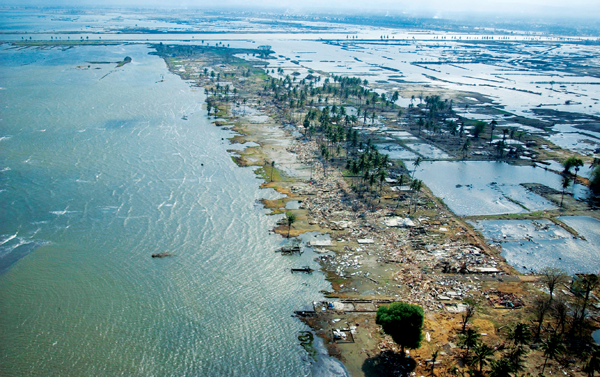
\includegraphics[width=0.7\textwidth]{./Pics/Examples/Coast_of_Banda_Aceh_2-12-05_050212-N-1450G-012.png}
		\caption{2004 Indian Ocean Tsunami (Banda Aceh)}
	\end{figure}
\end{frame}
\begin{frame}{Tsunamis}
	\begin{figure}
	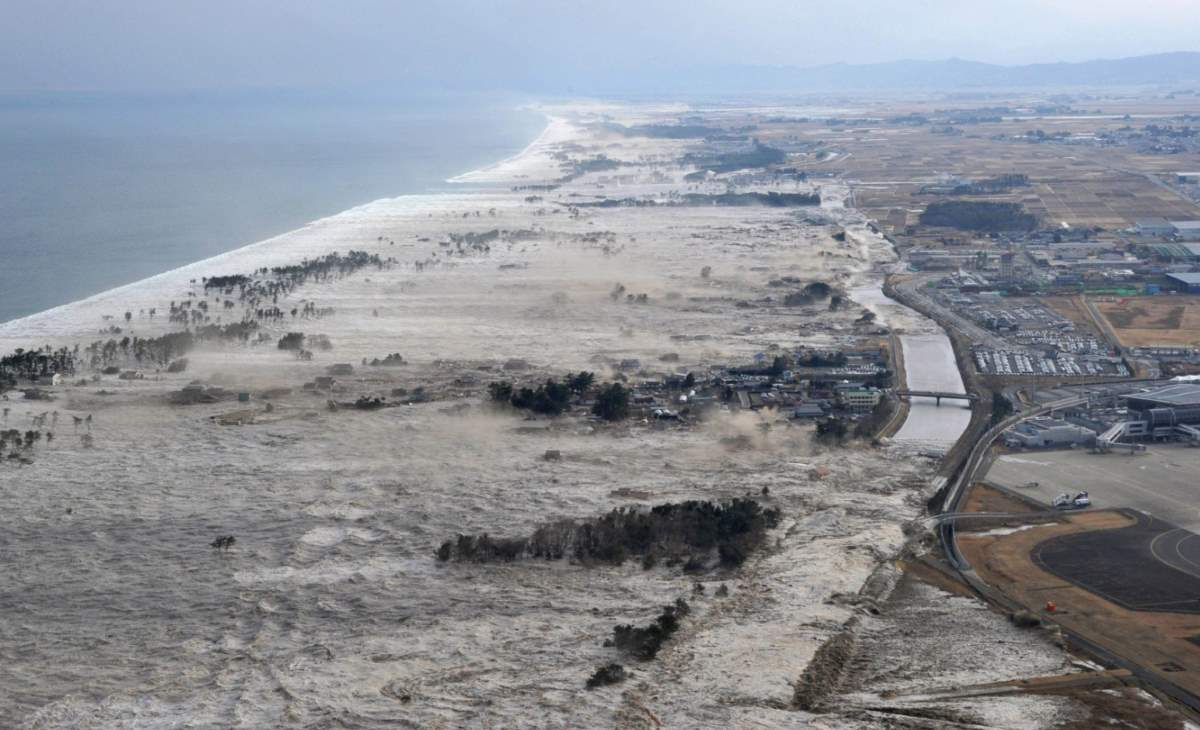
\includegraphics[width=0.7\textwidth]{./Pics/Examples/Tohoku-Tsunami.jpg}
	\caption{2011 Tohoku Tsunami}
	\end{figure}
\end{frame}

\againframe<3>{frame1}
\begin{frame}{Storm Surges}
		\begin{figure}
			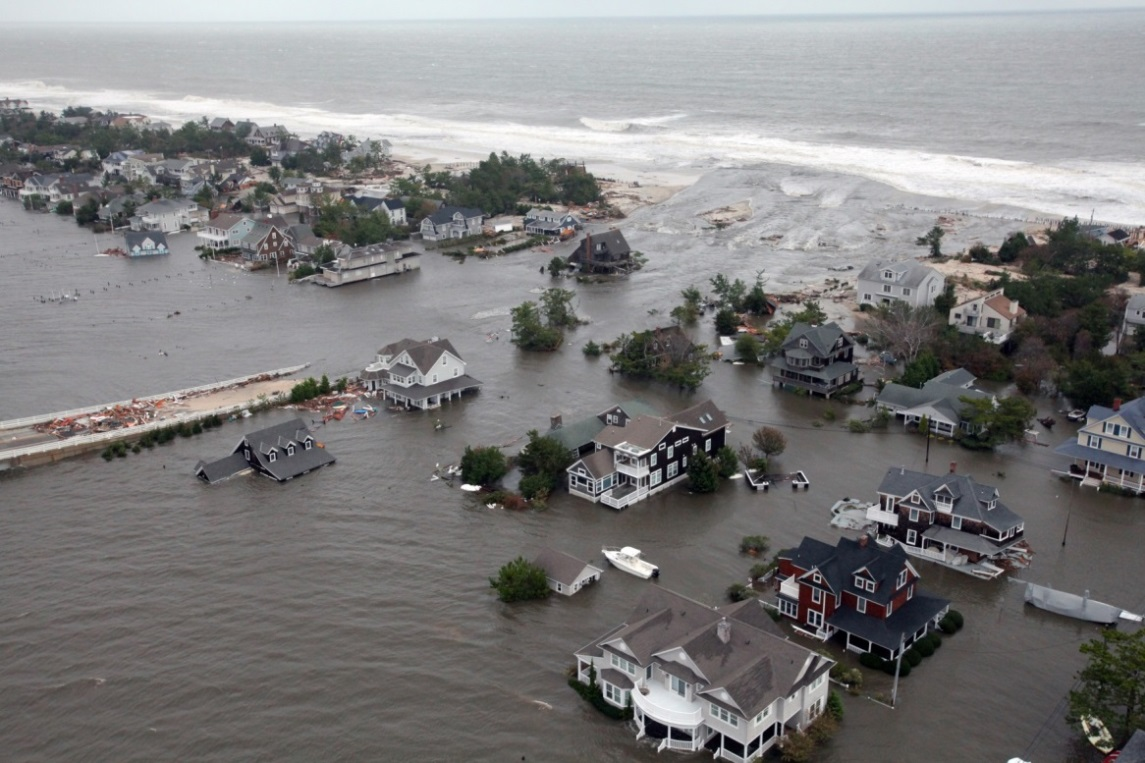
\includegraphics[width=0.7\textwidth]{./Pics/Examples/Sandy-storm-surge.jpg}
			\caption{2012 Hurricane Sandy Storm Surge}
		\end{figure}
\end{frame}
\againframe<4>{frame1}



\begin{frame}{Computational Modelling}
	%Picture Physical Process -> Mathematical Description -> Studying Mathematical Description (Numerical Solution)
	Goal: Model Physics On Computers \pause
	\begin{figure}
		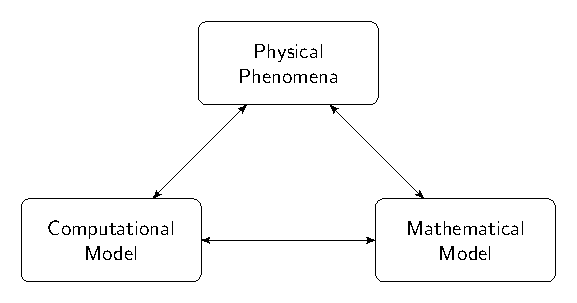
\includegraphics[width=\textwidth]{./Pics/ModelDiagrams/FlowChart.pdf}
	\end{figure}
\end{frame}

\section{History}
\begin{frame}{ANUGA}
	\begin{figure}
		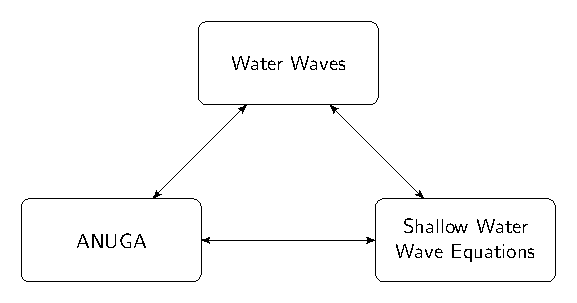
\includegraphics[width=\textwidth]{./Pics/ModelDiagrams/FlowChartANUGA.pdf}
	\end{figure}
\end{frame}

\begin{frame}{ANUGA: Water Waves}
	\begin{figure}
		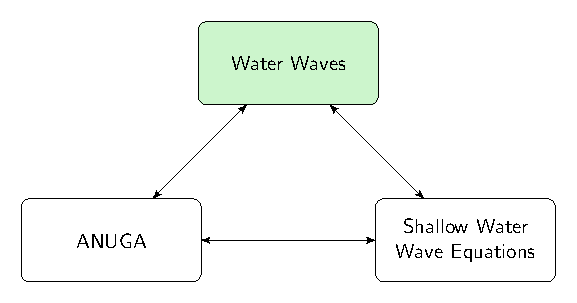
\includegraphics[width=\textwidth]{./Pics/ModelDiagrams/FlowChartANUGA1G.pdf}
	\end{figure}
	%main physical drivers
\end{frame}

\begin{frame}{ANUGA: Shallow Water Wave Equations}
	\begin{figure}
		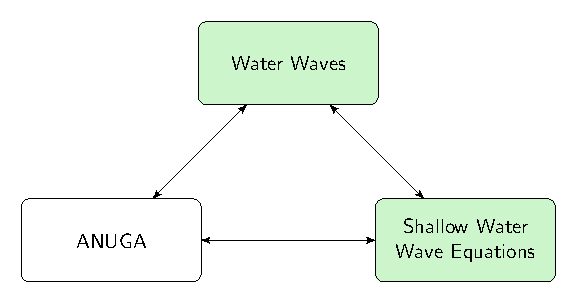
\includegraphics[width=\textwidth]{./Pics/ModelDiagrams/FlowChartANUGA12G.pdf}
	\end{figure}
	%main physical drivers it captures: nonlinearity and bed effects
\end{frame}

\begin{frame}{ANUGA}
	\begin{figure}
		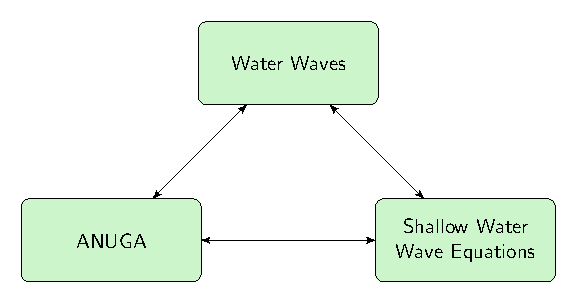
\includegraphics[width=\textwidth]{./Pics/ModelDiagrams/FlowChartANUGA123G.pdf}
	\end{figure}
\end{frame}


\begin{frame}{Outcome}
 New project at the ANU to develop a robust computational model for the Serre equations. \\
 
  \medskip
 \pause
 Goal:
 	\begin{figure}
 		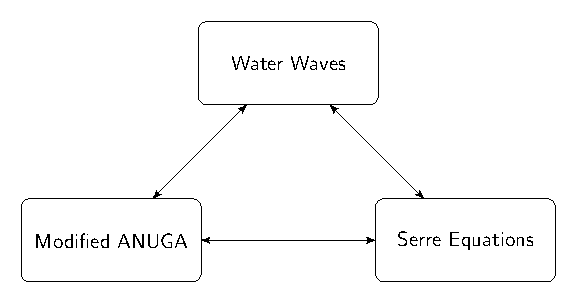
\includegraphics[width=\textwidth]{./Pics/ModelDiagrams/FlowChartSerre.pdf}
 	\end{figure}
\end{frame}
%mention previous work of ANU

\subsection{Serre Model}


\subsection{Serre Model}
\begin{frame}{Mathematical Model}
	%Picture Physical Process -> Mathematical Description -> Studying Mathematical Description (Numerical Solution)
	\begin{figure}
		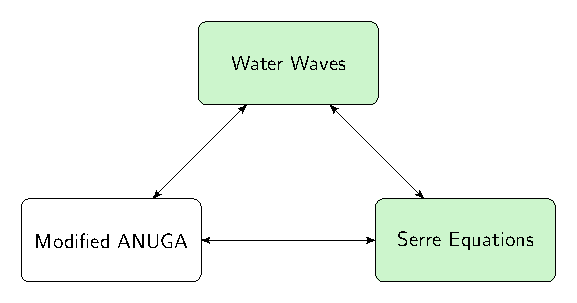
\includegraphics[width=\textwidth]{./Pics/ModelDiagrams/FlowChartSerre12G.pdf}
	\end{figure}
\end{frame}

\begin{frame}{Typical Scenario}
	%2D FLOW!!!!
	\begin{figure}
		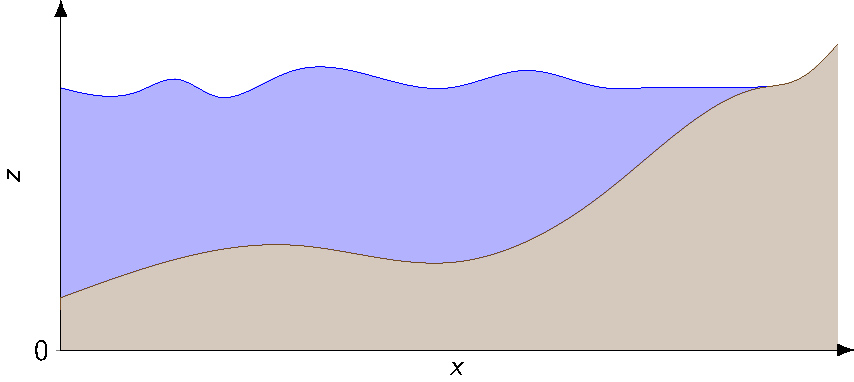
\includegraphics[width=\textwidth]{./Pics/WaterModelDiagrams/FressSurface.pdf}
	\end{figure}
\end{frame}
\begin{frame}{Navier Stokes Model}
	\begin{figure}
		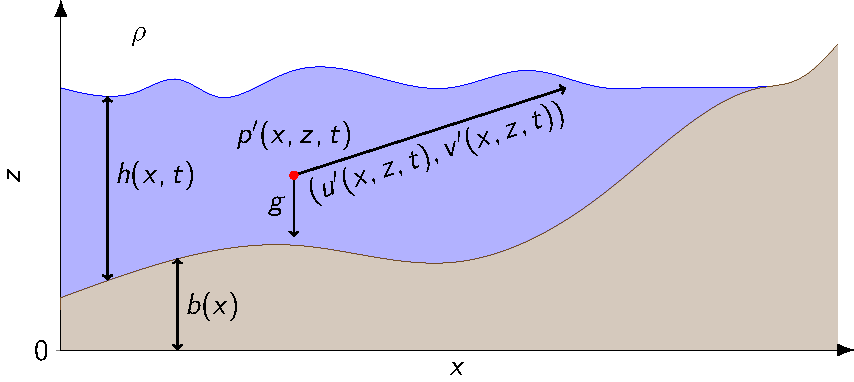
\includegraphics[width=\textwidth]{./Pics/WaterModelDiagrams/NavierStokes.pdf}
	\end{figure}
\end{frame}
\begin{frame}{Serre Model}
	\begin{figure}
		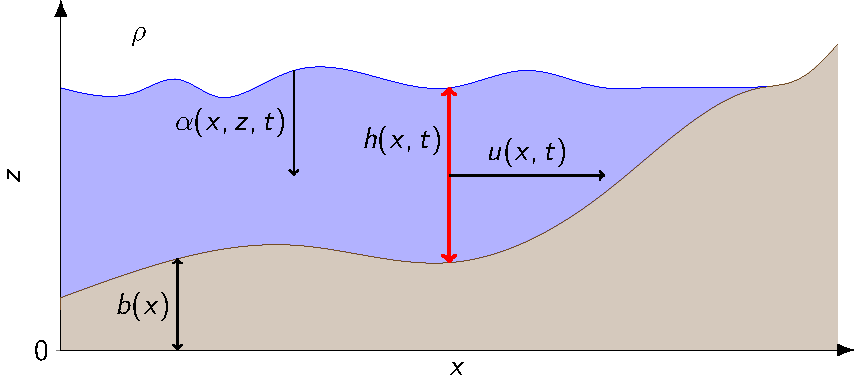
\includegraphics[width=\textwidth]{./Pics/WaterModelDiagrams/Serre.pdf}
	\end{figure}
\end{frame}
\begin{frame}{Assumptions}
	\bigbreak
	 \pause 
	 \begin{tabular}{l | c | c}
	 	Quantity& Shallow Water & Serre Equations\\
	 	& Wave Equations &\\
	 	\hline && \\
	 	Particle: $v'(x,z,t)$& $0$ & $u\frac{\partial b}{\partial x} - (z - b)\frac{\partial b}{\partial x}$ \\ & & \\ \pause
	 	Particle: $p'(x,z,t)$& $g\alpha$ & $g\alpha + \alpha{ \color{red}\Psi } + \frac{1}{2} \alpha \left(2h - \xi\right) { \color{blue} \Phi }$ \\ & & \\ \hline
	 \end{tabular}
	 \bigbreak
	  where $$\alpha(x,z,t) = (h(x,t) + b(x)) - z$$ \pause
	 \bigskip
	  and
		\begin{align*}
		&{ \color{red}\Psi }  = \dfrac{\partial b}{\partial x}\left(\dfrac{\partial u}{\partial t} + u\dfrac{\partial u}{\partial x} \right)  + u^2\dfrac{\partial^2 b}{\partial x^2}, &
		{ \color{blue} \Phi }  = \dfrac{\partial u }{\partial x} \dfrac{\partial u}{\partial x} -u \dfrac{\partial^2 u}{\partial x^2}  - \dfrac{\partial^2 u}{\partial x \partial t} .
		\end{align*}
\end{frame}
\begin{frame}{Equations}
	\begin{subequations}
		\begin{align*}
		&\text{Mass:} && \frac{\partial h}{\partial t} + \dfrac{\partial (uh)}{\partial x} = 0,  \\ \\
		&\text{Momentum:} &&\dfrac{\partial (uh)}{\partial t} + \dfrac{\partial}{\partial x} \left ( u^2h + \dfrac{gh^2}{2} + \dfrac{h^2}{2}{ \color{red}\Psi } + \dfrac{h^3}{3}{ { \color{blue} \Phi } }  \right )   \\ \\& &&\quad \quad \; \; +  \dfrac{\partial b}{\partial x} \left (gh +   h { \color{red}\Psi } + \dfrac{h^2}{2}{ { \color{blue} \Phi } }  \right ) = 0.
		\end{align*}
	\end{subequations}
		\begin{align*}
		&{ \color{red}\Psi }  = \dfrac{\partial b}{\partial x}\left(\dfrac{\partial u}{\partial t} + u\dfrac{\partial u}{\partial x} \right)  + u^2\dfrac{\partial^2 b}{\partial x^2}, &
		{ \color{blue} \Phi }  = \dfrac{\partial u }{\partial x} \dfrac{\partial u}{\partial x} -u \dfrac{\partial^2 u}{\partial x^2}  - \dfrac{\partial^2 u}{\partial x \partial t} .
		\end{align*}
\end{frame}
\begin{frame}{Pros and Cons}
	Pros:
	\begin{itemize}
		\item Includes dispersive effects
		\item Considered one of the best models for water waves
		\item Can apply techniques of ANUGA
	\end{itemize}
	Cons:
	\begin{itemize}
		\item More complex than the Shallow Water Wave Equations
	\end{itemize}
\end{frame}
\subsection{Computational Model for Serre Equations}
\begin{frame}{Computational Model}
	%Picture Physical Process -> Mathematical Description -> Studying Mathematical Description (Numerical Solution)
	\begin{figure}
		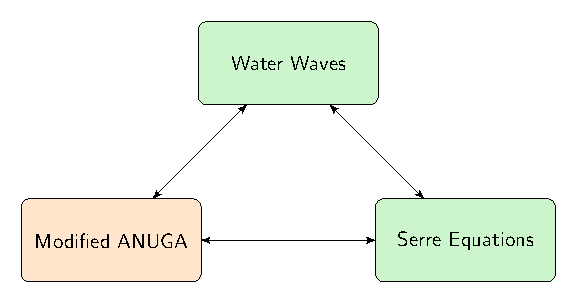
\includegraphics[width=\textwidth]{./Pics/ModelDiagrams/FlowChartSerre12G3O.pdf}
	\end{figure}
\end{frame}
\begin{frame}{Previous Work at the ANU}
	\begin{itemize}
		\item 2014: Chris Zoppou's PhD thesis  \\
			Demonstrated computational model for the 1D Serre equations.
		\item 2014: My Honours thesis \\
			Independent reproduction of Chris Zoppou's computational model
	\end{itemize}
	\pause
	Open problems:
	\begin{itemize}
		\item[2D:] Extension of the method to 2D equations
		\item[Robust:] Validation for steep gradients in free surface
		\item[Robust:] Inclusion and validation of dry beds
	\end{itemize}	
\end{frame}



\section{Thesis}
%Goal of thesis to develop numerical method that can handle dry beds and steep gradients using FEM and FVM

\begin{frame}{Thesis Goals}
	Solve these open problems:
	\begin{itemize}
		\item[2D:] 1D method that extends well to 2D
		\item[Robust:] Validation for steep gradients in free surface
		\item[Robust:] Inclusion and validation of dry beds
	\end{itemize}		
	\medskip
	\pause
	Technique: Develop a robust computational model from the 1D Serre equations that can be easily extended to 2D. 
\end{frame}

\section{Thesis: Method}
\begin{frame}{Method}
	%Brief
	\begin{itemize}
		\item Finite Volume Method (ANUGA)
		\item Finite Element Method
	\end{itemize}
\end{frame}
\subsection{Finite Volume Method}
\begin{frame}{Finite Volume Method}
\begin{itemize}
	\item[2D:] Extends well to 2D
	\item[Robust:] Stable in the presence of steep gradients
	\item[Robust:] Stable in the presence of dry beds
	\item Maintains conservation properties of the equations
\end{itemize}
\pause  Chris Zoppou's thesis demonstrated an adaptation of the Finite Volume Method to solve the Serre Equations.
\end{frame}

\begin{frame}{Equations}
		\begin{subequations}
			\begin{align*}
			&\frac{\partial h}{\partial t} + \dfrac{\partial (uh)}{\partial x} = 0,  \\ \\
			&\dfrac{\partial (uh)}{\partial t} + \dfrac{\partial}{\partial x} \left ( u^2h + \dfrac{gh^2}{2} + \dfrac{h^2}{2}{ \color{red}\Psi } + \dfrac{h^3}{3}{ { \color{blue} \Phi } }  \right )  +  \dfrac{\partial b}{\partial x} \left (gh +   h { \color{red}\Psi } + \dfrac{h^2}{2}{ { \color{blue} \Phi } }  \right ) = 0
			\end{align*}
		\end{subequations}
				\begin{align*}
				&{ \color{red}\Psi }  = \dfrac{\partial b}{\partial x}\left(\dfrac{\partial u}{\partial t} + u\dfrac{\partial u}{\partial x} \right)  + u^2\dfrac{\partial^2 b}{\partial x^2}, &
				{ \color{blue} \Phi }  = \dfrac{\partial u }{\partial x} \dfrac{\partial u}{\partial x} -u \dfrac{\partial^2 u}{\partial x^2}  - \dfrac{\partial^2 u}{\partial x \partial t} .
				\end{align*}
	\pause
	For a Finite Volume Method we require equations in the form
	\begin{equation*}
	\frac{\partial q}{\partial t} + \frac{\partial f(q)}{\partial x} + s(q) = 0
	\end{equation*}
	where $f(q)$ and $s(q)$ do not contain temporal derivatives
\end{frame}

\begin{frame}{Equations}
	\begin{subequations}
		\begin{align*}
		& {\color{blue}\frac{\partial h}{\partial t}} + \dfrac{\partial (uh)}{\partial x} = 0,  \\ \\
		& {\color{blue}\dfrac{\partial (uh)}{\partial t}} + \dfrac{\partial}{\partial x} \left ( u^2h + \dfrac{gh^2}{2} + \dfrac{h^2}{2}{\Psi } + \dfrac{h^3}{3}{ { \Phi } }  \right )  +  \dfrac{\partial b}{\partial x} \left (gh +   h {\Psi } + \dfrac{h^2}{2}{ {  \Phi } }  \right ) = 0
		\end{align*}
	\end{subequations}
	\begin{align*}
	&{ \Psi }  = \dfrac{\partial b}{\partial x}\left(\dfrac{\partial u}{\partial t} + u\dfrac{\partial u}{\partial x} \right)  + u^2\dfrac{\partial^2 b}{\partial x^2}, &
	{  \Phi }  = \dfrac{\partial u }{\partial x} \dfrac{\partial u}{\partial x} -u \dfrac{\partial^2 u}{\partial x^2}  - \dfrac{\partial^2 u}{\partial x \partial t} .
	\end{align*}

	For a Finite Volume Method we require equations in the form
	\begin{equation*}
	{\color{blue}\frac{\partial q}{\partial t}} + \frac{\partial f(q)}{\partial x} + s(q) = 0
	\end{equation*}
	where $f(q)$ and $s(q)$ do not contain temporal derivatives
\end{frame}

\begin{frame}{Equations}
	\begin{subequations}
		\begin{align*}
		& {\color{blue}\frac{\partial h}{\partial t}} + {\color{red}\dfrac{\partial (uh)}{\partial x}} = 0,  \\ \\
		& {\color{blue}\dfrac{\partial (uh)}{\partial t}} +  {\color{red}\dfrac{\partial}{\partial x} \left ( u^2h + \dfrac{gh^2}{2} + \dfrac{h^2}{2}{\Psi } + \dfrac{h^3}{3}{ { \Phi } }  \right ) }  +  \dfrac{\partial b}{\partial x} \left (gh +   h {\Psi } + \dfrac{h^2}{2}{ {  \Phi } }  \right ) = 0
		\end{align*}
	\end{subequations}
	\begin{align*}
	&{ \Psi }  = \dfrac{\partial b}{\partial x}\left(\dfrac{\partial u}{\partial t} + u\dfrac{\partial u}{\partial x} \right)  + u^2\dfrac{\partial^2 b}{\partial x^2}, &
	{  \Phi }  = \dfrac{\partial u }{\partial x} \dfrac{\partial u}{\partial x} -u \dfrac{\partial^2 u}{\partial x^2}  - \dfrac{\partial^2 u}{\partial x \partial t} .
	\end{align*}
	
	For a Finite Volume Method we require equations in the form
	\begin{equation*}
	{\color{blue}\frac{\partial q}{\partial t}} +  {\color{red}\frac{\partial f(q)}{\partial x}} + s(q) = 0
	\end{equation*}
	where $f(q)$ and $s(q)$ do not contain temporal derivatives
\end{frame}

\begin{frame}{Equations}
	\begin{subequations}
		\begin{align*}
		& {\color{blue}\frac{\partial h}{\partial t}} + {\color{red}\dfrac{\partial (uh)}{\partial x}} = 0,  \\ \\
		& {\color{blue}\dfrac{\partial (uh)}{\partial t}} +  {\color{red}\dfrac{\partial}{\partial x} \left ( u^2h + \dfrac{gh^2}{2} + \dfrac{h^2}{2}{\Psi } + \dfrac{h^3}{3}{ { \Phi } }  \right ) }  +  {\color{green!50!black}\dfrac{\partial b}{\partial x} \left (gh +   h {\Psi } + \dfrac{h^2}{2}{ {  \Phi } }  \right )} = 0
		\end{align*}
	\end{subequations}
	\begin{align*}
	&{ \Psi }  = \dfrac{\partial b}{\partial x}\left(\dfrac{\partial u}{\partial t} + u\dfrac{\partial u}{\partial x} \right)  + u^2\dfrac{\partial^2 b}{\partial x^2}, &
	{  \Phi }  = \dfrac{\partial u }{\partial x} \dfrac{\partial u}{\partial x} -u \dfrac{\partial^2 u}{\partial x^2}  - \dfrac{\partial^2 u}{\partial x \partial t} .
	\end{align*}
	
	For a Finite Volume Method we require equations in the form
	\begin{equation*}
	{\color{blue}\frac{\partial q}{\partial t}} +  {\color{red}\frac{\partial f(q)}{\partial x}} +  {\color{green!50!black} s(q) } = 0
	\end{equation*}
	where $f(q)$ and $s(q)$ do not contain temporal derivatives
\end{frame}

\begin{frame}{Reformulation}
	\begin{align*}
	& \frac{\partial h}{\partial t} + \dfrac{\partial (uh)}{\partial x} = 0,  \\ \nonumber \\
	\begin{split}
	\frac{\partial G}{\partial t}  + \frac{\partial}{\partial x} \left( {u} G + \frac{gh^2}{2} - \frac{2}{3}h^3 \left[\frac{\partial {u}}{\partial x}\right]^2 + h^2 {u}\frac{\partial {u}}{\partial x}\frac{\partial b}{\partial x} \right) \\ + \frac{1}{2}h^2 {u} \frac{\partial {u}}{\partial x} \frac{\partial^2 b}{\partial x^2}  - h {u}^2\frac{\partial b}{\partial x}\frac{\partial^2 b}{\partial x^2} + gh\frac{\partial b}{\partial x} = 0 .
	\end{split}
	\end{align*}
	with
	\[ G =  h {u} \left(1 + \frac{\partial h}{\partial x}\frac{\partial b}{\partial x} + \frac{1}{2}h\frac{\partial^2 b}{\partial x^2} + \left[\frac{\partial b}{\partial x}\right]^2 \right) - \frac{\partial}{\partial x}\left(\frac{1}{3}h^3  \frac{\partial {u}}{\partial x}\right).\]
	%Correct form
	\blfootnote{Zoppou, C. (2014).
		Numerical Solution of the One-dimensional and Cylindrical
		Serre Equations for Rapidly Varying Free Surface Flows. PhD thesis, Australian National University.}
\end{frame}

\begin{frame}{Reformulation}
	\begin{align*}
	& {\color{blue}\frac{\partial h}{\partial t}} + {\color{red}\dfrac{\partial (uh)}{\partial x}} = 0,  \\ \nonumber \\
	\begin{split}
	{\color{blue}\frac{\partial G}{\partial t} }  + {\color{red}\frac{\partial}{\partial x} \left( {u} G + \frac{gh^2}{2} - \frac{2}{3}h^3 \left[\frac{\partial {u}}{\partial x}\right]^2 + h^2 {u}\frac{\partial {u}}{\partial x}\frac{\partial b}{\partial x} \right)} \\ + {\color{green!50!black}\frac{1}{2}h^2 {u} \frac{\partial {u}}{\partial x} \frac{\partial^2 b}{\partial x^2}  - h {u}^2\frac{\partial b}{\partial x}\frac{\partial^2 b}{\partial x^2} + gh\frac{\partial b}{\partial x} } = 0 .
	\end{split}
	\end{align*}
	with
	\[ G =  h {u} \left(1 + \frac{\partial h}{\partial x}\frac{\partial b}{\partial x} + \frac{1}{2}h\frac{\partial^2 b}{\partial x^2} + \left[\frac{\partial b}{\partial x}\right]^2 \right) - \frac{\partial}{\partial x}\left(\frac{1}{3}h^3  \frac{\partial {u}}{\partial x}\right).\]
	%Correct form
	\blfootnote{Zoppou, C. (2014).
		Numerical Solution of the One-dimensional and Cylindrical
		Serre Equations for Rapidly Varying Free Surface Flows. PhD thesis, Australian National University.}
\end{frame}

\begin{frame}{Finite Volume Example}	
	\begin{equation*}
	{\color{blue}\frac{\partial q}{\partial t}} + {\color{red}\frac{\partial f(q)}{\partial x} } + {\color{green!40!black} s(q) } = 0
	\end{equation*}	
	\pause
	Integrate from $t^0$ to $t^1$
	\begin{multline*}
	{ \color{blue}q(x,t^1)} {\color{blue}-} { {\color{blue} q(x,t^0) } }+   { {\color{red}\int_{t^0}^{t^1}  \frac{\partial f(q)}{\partial x} \; dt}}   +   {\color{green!40!black}\int_{t^0}^{t^1}  s(q(x,t)) \; dt }
	\end{multline*}
	\pause
	Integrate over $C_2 = [x_{3/2}, x_{5/2}]$  
	\begin{multline*}
	{ {\color{blue}\int_{C_2} q(x,t^1) \; dx}} {\color{blue}-} { {\color{blue}\int_{C_2} q(x,t^0) \; dx } } +  \bigg(  {\color{red}\int_{t^0}^{t^1} f(q(x_{5/2},t)) \; dt} \\ {\color{red}-} {{\color{red}\int_{t^0}^{t^1} f(q(x_{3/2},t)) \; dt}}\bigg) +  { {\color{green!40!black}\int_{t^0}^{t^1} \int_{C_2} s(q(x,t)) \; dt \; dx }}
	\end{multline*}
\end{frame}

\begin{frame}{Finite Volume Example}	
	\begin{multline*}
	{ {\color{blue}\int_{C_2} q(x,t^1) \; dx}} {\color{blue}-} { {\color{blue}\int_{C_2} q(x,t^0) \; dx } } +  \bigg(  {\color{red}\int_{t^0}^{t^1} f(q(x_{5/2},t)) \; dt} \\ {\color{red}-} {{\color{red}\int_{t^0}^{t^1} f(q(x_{3/2},t)) \; dt}}\bigg) +  { {\color{green!40!black}\int_{t^0}^{t^1} \int_{C_2} s(q(x,t)) \; dt \; dx }}
	\end{multline*}
	\pause
	\begin{multline*}
	\overbrace{ {\color{blue}\int_{C_2} q(x,t^1) \; dx}}^{\overline{q}^1_2} {\color{blue}-} \overbrace{ {\color{blue}\int_{C_2} q(x,t^0) \; dx } }^{\overline{q}^0_2} +  \bigg( \overbrace{ {\color{red}\int_{t^0}^{t^1} f(q(x_{5/2},t)) \; dt}}^{F^0_{\frac{5}{2}}} \\ {\color{red}-} \overbrace{{\color{red}\int_{t^0}^{t^1} f(q(x_{3/2},t)) \; dt}}^{F^0_{\frac{3}{2}}}  \bigg) +  \overbrace{ {\color{green!40!black}\int_{t^0}^{t^1} \int_{C_2} s(q(x,t)) \; dt }}^{S^0_{2}}
	\end{multline*}
	\pause 
	\begin{equation*}
	{\color{blue}\overline{q}^1_2 } = {\color{blue}\overline{q}^0_2} - \left(  {\color{red}F^0_{\frac{5}{2}} - F^0_{\frac{3}{2}} } \right) -  \left({\color{green!40!black}S^0_2}\right)
	\end{equation*}	
\end{frame}

\begin{frame}{Finite Volume Example}	
	\begin{multline*}
	\overbrace{ {\color{blue}\int_{C_2} q(x,t^1) \; dx}}^{\overline{q}^1_2} {\color{blue}-} \overbrace{ {\color{blue}\int_{C_2} q(x,t^0) \; dx } }^{\overline{q}^0_2} +  \bigg( \overbrace{ {\color{red}\int_{t^0}^{t^1} f(q(x_{5/2},t)) \; dt}}^{F^0_{\frac{5}{2}}} \\ {\color{red}-} \overbrace{{\color{red}\int_{t^0}^{t^1} f(q(x_{3/2},t)) \; dt}}^{F^0_{\frac{3}{2}}}  \bigg) +  \overbrace{ {\color{green!40!black}\int_{t^0}^{t^1} \int_{C_2} s(q(x,t)) \; dt }}^{S^0_{2}}
	\end{multline*}
	\pause 
	\begin{equation*}
	{\color{blue}\overline{q}^1_2 } = {\color{blue}\overline{q}^0_2} - \left(  {\color{red}F^0_{\frac{5}{2}} - F^0_{\frac{3}{2}} } \right) -  \left({\color{green!40!black}S^0_2}\right)
	\end{equation*}	
\end{frame}
\begin{frame}{Function at $t=t^0$}
	\begin{figure}
		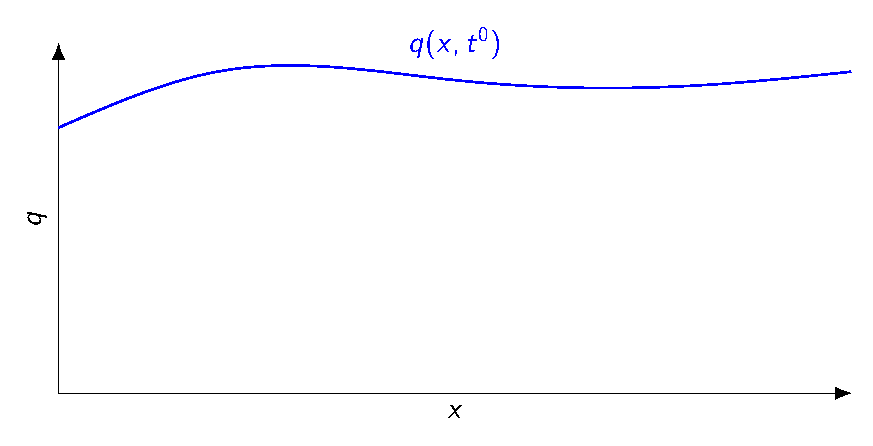
\includegraphics[width=\textwidth]{./Pics/FVMpicture/Function.pdf}
	\end{figure}
\end{frame}
\begin{frame}{Cell Discretisation}
	\begin{figure}
		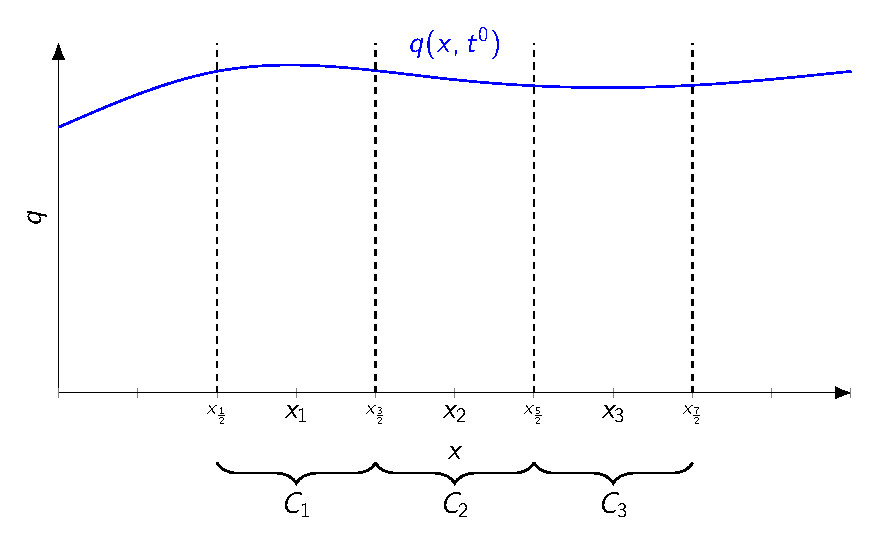
\includegraphics[width=\textwidth]{./Pics/FVMpicture/Cells.pdf}
	\end{figure}
\end{frame}
\begin{frame}{Total Amount}
	\begin{figure}
		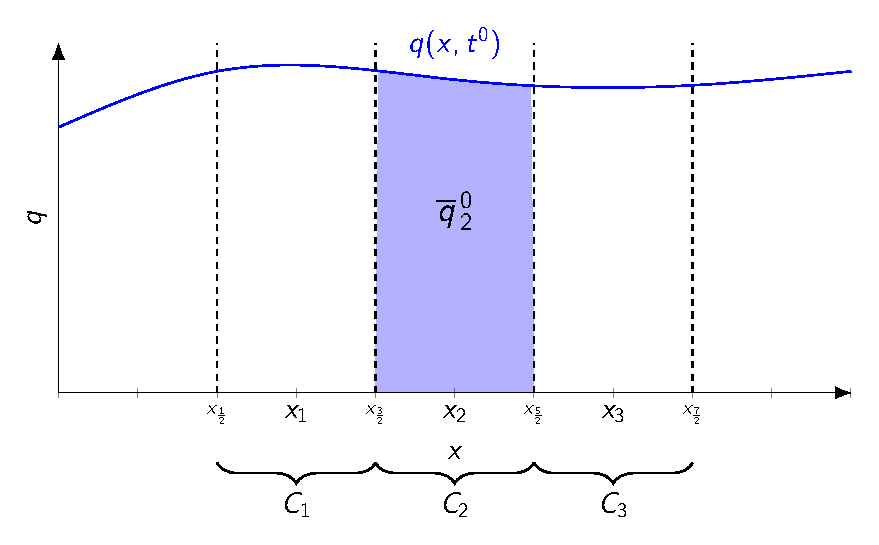
\includegraphics[width=0.9\textwidth]{./Pics/FVMpicture/Total.pdf}
	\end{figure}
\end{frame}
\begin{frame}{Flux Left}
	\begin{figure}
		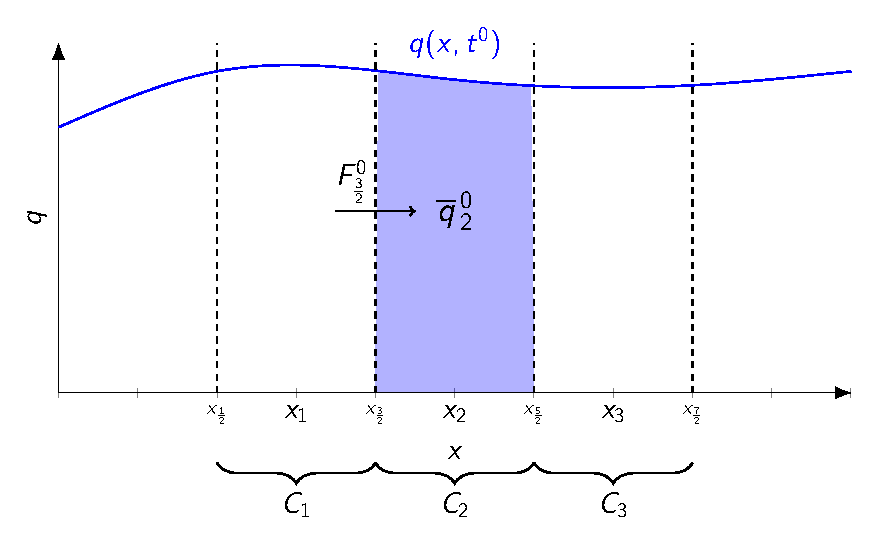
\includegraphics[width=\textwidth]{./Pics/FVMpicture/TotalFluxIn.pdf}
	\end{figure}
\end{frame}
\begin{frame}{Flux Right}
	\begin{figure}
		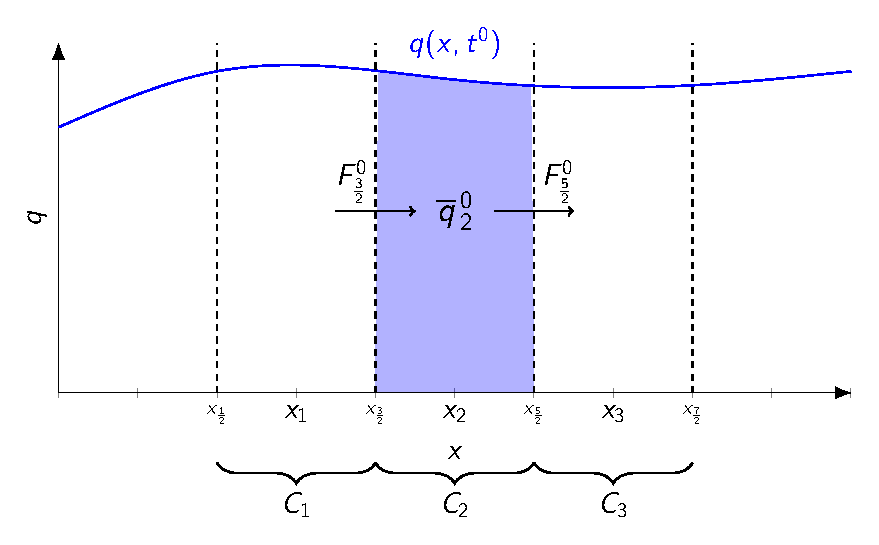
\includegraphics[width=\textwidth]{./Pics/FVMpicture/TotalFluxInOut.pdf}
	\end{figure}
\end{frame}
\begin{frame}{Source}
	\begin{figure}
		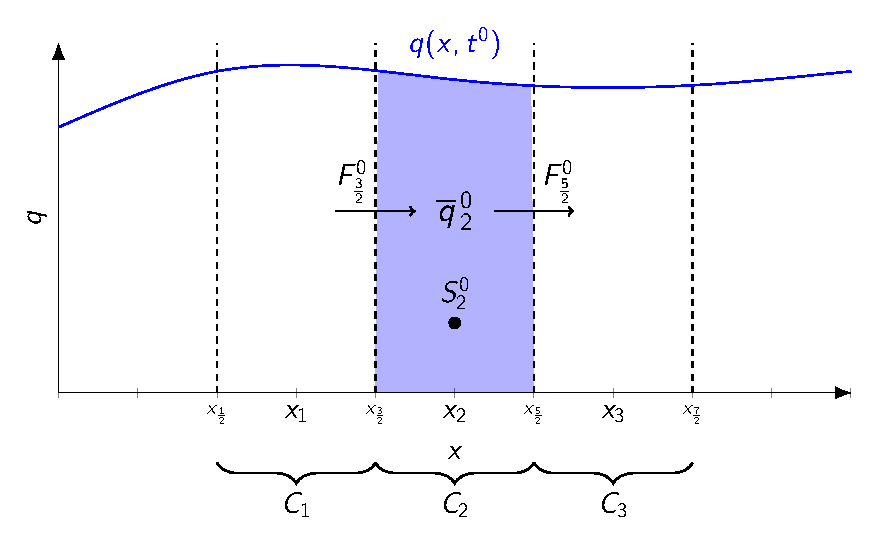
\includegraphics[width=\textwidth]{./Pics/FVMpicture/TotalFluxInOutSource.pdf}
	\end{figure}
\end{frame}


\begin{frame}{Update Formula for Serre Equations}
	\begin{equation*}
	\overline{h}_j^{n+1} = \overline{h}_j^n -  \left[F_{j + 1/2}^n - F_{j - 1/2}^n \right]
	\end{equation*}
	\begin{equation*}
	\overline{G}_j^{n+1}  = \overline{G}_j^n -  \left[F_{j + 1/2}^n - F_{j - 1/2}^n \right] -  S^n_j
	\end{equation*}
	\pause
	\begin{itemize}
		\item All the fluxes $F^n_{j + 1/2}$ and $F^n_{j - 1/2}$ and the source term $ S^n_j$ require $u$ at $t^n$
	\end{itemize}
	
\end{frame}

\subsection{Finite Element Method}
\begin{frame}{Calculate Velocity}
		\[ G =  h {u} \left(1 + \frac{\partial h}{\partial x}\frac{\partial b}{\partial x} + \frac{1}{2}h\frac{\partial^2 b}{\partial x^2} + \left[\frac{\partial b}{\partial x}\right]^2 \right) - \frac{\partial}{\partial x}\left(\frac{1}{3}h^3  \frac{\partial {u}}{\partial x}\right).\]
		\pause
		\begin{itemize}
			\item Previously used a Finite Difference Method \footnote{Zoppou, C. (2014).
				Numerical Solution of the One-dimensional and Cylindrical
				Serre Equations for Rapidly Varying Free Surface Flows. PhD thesis, Australian National University.}
			\item Contribution: use a Finite Element Method
		\end{itemize}
\end{frame}

\begin{frame}{Finite Element Method}
	%mention dry beds
	\begin{itemize}
		\item[2D:] Extends well to 2D
		\item[Robust:] Stable in the presence of steep gradients 
		\item Maintains conservation properties
	\end{itemize}
\end{frame}

\begin{frame}{Finite Element Method Example}
	Example:
		\[  -\frac{\partial^2 {u}}{\partial x^2}= f\]
		\pause
	Weak Form:
	\[
	 -\int_{\Omega }\frac{\partial^2 {u}}{\partial x^2} v \; dx = \int_{\Omega } f v \; dx
	\]
	\pause
	Integrate by parts %(Dirichlet boundary conditions):
	\[
  \int_{\Omega }\frac{\partial {u}}{\partial x} \frac{\partial {v}}{\partial x} \; dx  = \int_{\Omega } f v \; dx
	\]
\end{frame}

\begin{frame}<1-2>[label=frame2]{Finite Element Method}
	\[
	 \int_{\Omega }\frac{\partial {u}}{\partial x} \frac{\partial {v}}{\partial x} \; dx  = \int_{\Omega } f v \; dx
	\]
	\pause
	\[
	 \sum_j  \left[\int_{C_j} \frac{\partial {u}}{\partial x} \frac{\partial {v}}{\partial x} \; dx \right] = \sum_j \left[ \int_{C_j} f v  \; dx \right]
	\]
	\pause
		\[
		\sum_j  \left[\int_{C_j} \frac{\partial {\hat{u}_j }}{\partial x} \frac{\partial {\hat{v}_j }}{\partial x} \; dx\right]  = \sum_j \left[ \int_{C_j} \hat{f}_j \hat{v}_j  \; dx \right]
		\]
	\pause
		\begin{equation*}
		\boldsymbol{A} \vec{u} = \vec{c}
		\end{equation*}
	\pause
		where 
		\begin{itemize}
			\item $\boldsymbol{A}$ depends on $\hat{v}_j$
			\item $\vec{u}$ determines $\hat{u}_j$
			\item $\vec{c}$ depends on $\hat{f}_j$ and $\hat{v}_j$
		\end{itemize}
\end{frame}

\begin{frame}{Piecewise Polynomial Representation}
	\begin{figure}
		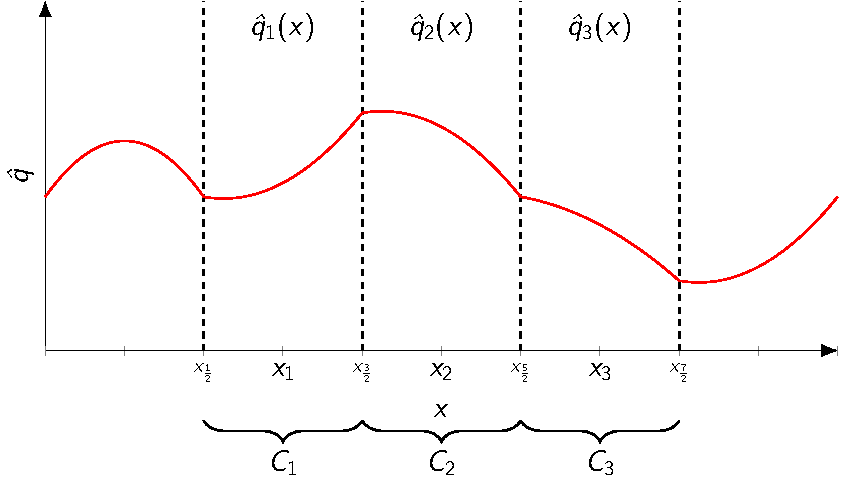
\includegraphics[width=\textwidth]{./Pics/PolyRep/P2.pdf}
	\end{figure}
\end{frame}

\againframe<3-5>{frame2}

\begin{frame}{Finite Element Method for Serre Equations}
		\[ G =  h {u} \left(1 + \frac{\partial h}{\partial x}\frac{\partial b}{\partial x} + \frac{1}{2}h\frac{\partial^2 b}{\partial x^2} + \left[\frac{\partial b}{\partial x}\right]^2 \right) - \frac{\partial}{\partial x}\left(\frac{1}{3}h^3  \frac{\partial {u}}{\partial x}\right)\]
	\pause
	\begin{equation*}
	\boldsymbol{A} \vec{u} = \vec{c}
	\end{equation*}
	where 
	\begin{itemize}
		\item $\boldsymbol{A}$ depends on the polynomial representation of $h$, $b$ and test function
		\item $\vec{u}$ determines the polynomial representation of $u$
		\item $\vec{c}$ depends on polynomial representation of $G$ and test function
	\end{itemize}
\end{frame}


\begin{frame}{Method}
		\begin{figure}
			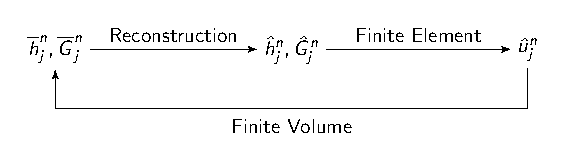
\includegraphics[width=\textwidth]{./Pics/ModelDiagrams/FlowChartNoBox.pdf}
		\end{figure}
\end{frame}

\begin{frame}{Progress}
	\begin{itemize}
		\item[2D:] 1D method that extends well to 2D \checkmark
		\item[Robust:] Validation for steep gradients in free surface
		\item[Robust:] Inclusion and validation of dry beds
	\end{itemize}	
\end{frame}

\section{Thesis: Validation}
\begin{frame}{Validation}
	%Brief
	\begin{itemize}
		\item Steep gradients in the free surface
		\item Dry beds
	\end{itemize}
\end{frame}


\subsection{ Model Validation for Steep Gradients in the Flow}
\begin{frame}{Statement of Problem}
	How does this initially still body of water evolve?
	\begin{figure}
		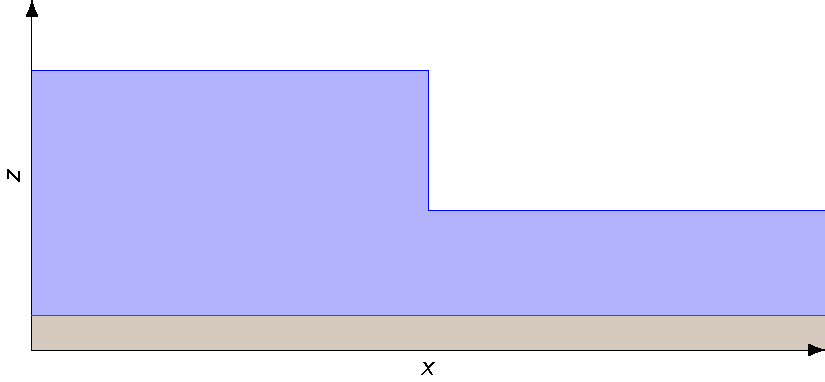
\includegraphics[width=\textwidth]{./Pics/SteepGradients/Wavetank.pdf}
	\end{figure}
\end{frame}	

\begin{frame}{Our New Numerical Solution}
	\begin{figure}
		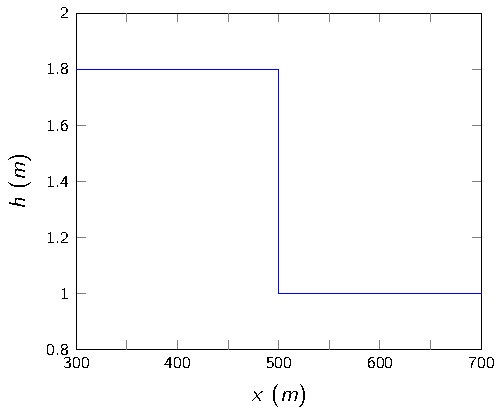
\includegraphics[width=0.5\textwidth]{./Pics/SteepGradients/DBinit.pdf}
		\pause
		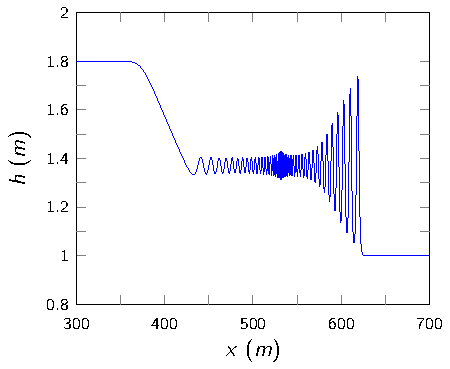
\includegraphics[width=0.5\textwidth]{./Pics/SteepGradients/DBfint.pdf}
	\end{figure}
	\blfootnote{Pitt, J., Zoppou, C., and Roberts, S. (2018).
		Behaviour of the Serre Equations in the Presence of Steep
		Gradients Revisited.
		Wave Motion, 76(1):61–77.}
\end{frame}

%What was known
%Previous Work
%Improvements
\begin{frame}{What was known}
	\begin{itemize}
		\item No analytic solutions
		\item Some experimental comparisons \footnote{Zoppou, C. (2014).
			Numerical Solution of the One-dimensional and Cylindrical
			Serre Equations for Rapidly Varying Free Surface Flows. PhD thesis, Australian National University.}
		\item Other numerical solutions from the literature
		\end{itemize}
\end{frame}

\begin{frame}{Contribution}
	\blfootnote{Pitt, J., Zoppou, C., and Roberts, S. (2018).
		Behaviour of the Serre Equations in the Presence of Steep
		Gradients Revisited.
		Wave Motion, 76(1):61–77.}
	\begin{itemize}
		\item Observed this new behaviour
		\item Demonstrated convergence
		\item Comprehensive review of numerical solutions from the literature
	\end{itemize}
	
\end{frame}

\begin{frame}{Convergence}
As we increase number of cells the numerical solutions should converge to the true solution
\end{frame}
\begin{frame}{Convergence}
		\begin{figure}
			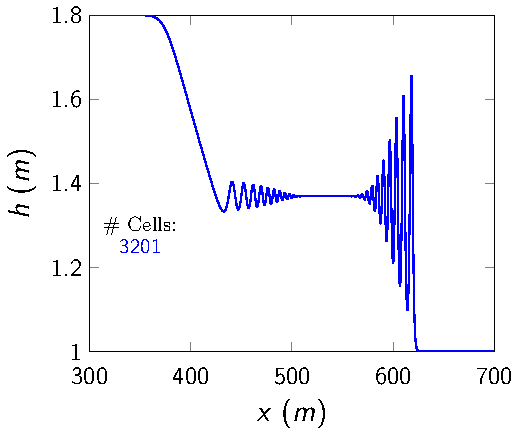
\includegraphics[width=0.8\textwidth]{./Pics/SteepGradients/h0.pdf}
		\end{figure}
\end{frame}
\begin{frame}{Convergence}
		\begin{figure}
			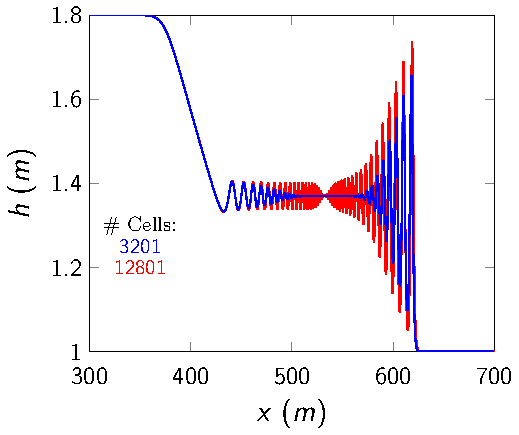
\includegraphics[width=0.8\textwidth]{./Pics/SteepGradients/h01.pdf}
		\end{figure}
\end{frame}
\begin{frame}{Convergence}
		\begin{figure}
			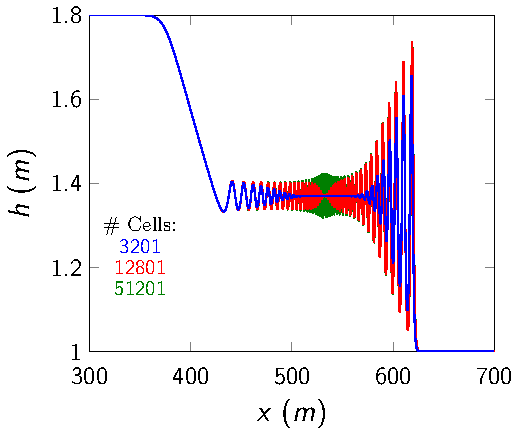
\includegraphics[width=0.8\textwidth]{./Pics/SteepGradients/h012.pdf}
		\end{figure}
\end{frame}
\begin{frame}{Convergence}
		\begin{figure}
			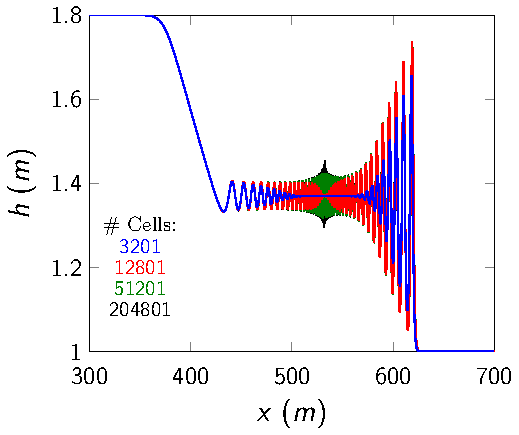
\includegraphics[width=0.8\textwidth]{./Pics/SteepGradients/h0123.pdf}
		\end{figure}
\end{frame}


\begin{frame}{Comprehensive Review}
	\begin{itemize}
		\item Demonstrated consistent behaviour across many numerical methods
		\item Were able to explain why the behaviour had not previously been observed
	\end{itemize}
\end{frame}

\begin{frame}{Result}
	Validated our computational model when steep gradients are present in the free surface. \footnote{Pitt, J., Zoppou, C., and Roberts, S. (2018).
		Behaviour of the Serre Equations in the Presence of Steep
		Gradients Revisited.
		Wave Motion, 76(1):61–77.}
\end{frame}

\begin{frame}{Progress}
	\begin{itemize}
		\item[2D:] 1D method that extends well to 2D \checkmark
		\item[Robust:] Validation for steep gradients in free surface \checkmark
		\item[Robust:] Inclusion and validation of dry beds
	\end{itemize}
\end{frame}

\subsection{Solution in the Presence of Dry Beds}
%What was known
%Previous Work
%Improvements
\begin{frame}{Statement of Problem}
	Properly handle interaction of waves and the dry bed
		\begin{figure}
			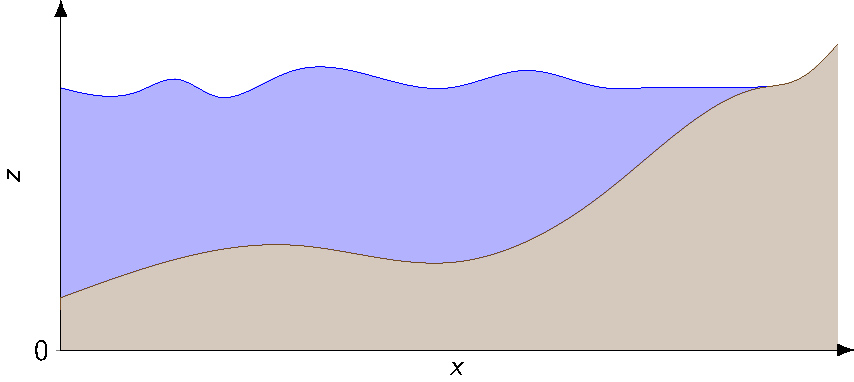
\includegraphics[width=\textwidth]{./Pics/WaterModelDiagrams/FressSurface.pdf}
		\end{figure}
\end{frame}

\begin{frame}{What was known}
	\begin{itemize}
		\item No analytic solutions
		\item A variety of numerical techniques only compared to experimental data
	\end{itemize}
\end{frame}

\begin{frame}{Contribution}
	\begin{itemize}
		\item Solved modified equations that did possess analytic solutions
		\item Compared with experimental data
	\end{itemize}
\end{frame}

\begin{frame}{Constructing Modified Equations}
	\begin{itemize}
		\item Pick functions for height, velocity and bed: $h^*$, $u^*$ and $b^*$
		\item Add source terms to Serre equations that force $h^*$, $u^*$ and $b^*$ to be solutions
		\item Validation tests
	\end{itemize}
\end{frame}
\begin{frame}{Pick Functions}

\begin{figure}
	\centering
	\begin{subfigure}{0.5\textwidth}
		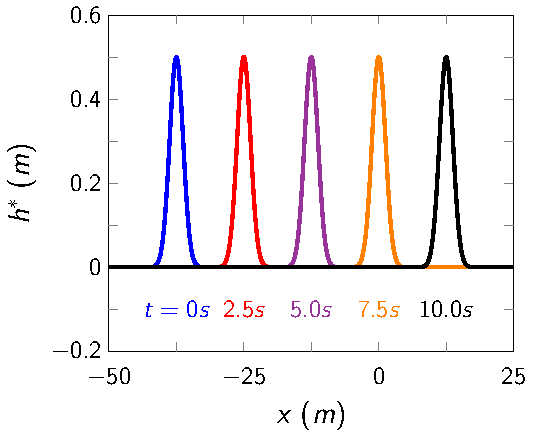
\includegraphics[width=0.8\textwidth]{./Pics/DryBed/Forced/h.pdf}
	\end{subfigure}%
	\begin{subfigure}{0.5\textwidth}
		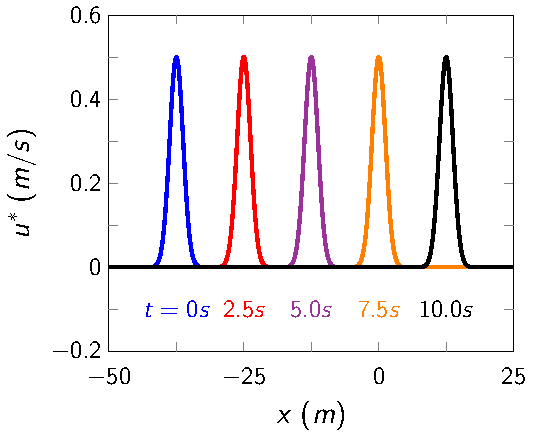
\includegraphics[width=0.8\textwidth]{./Pics/DryBed/Forced/u.pdf}
	\end{subfigure}
	\begin{subfigure}{0.5\textwidth}
		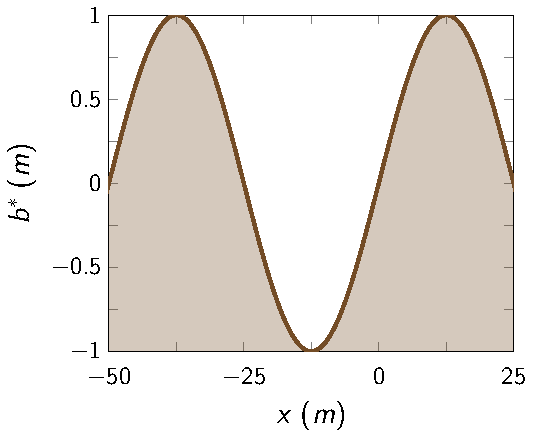
\includegraphics[width=0.8\textwidth]{./Pics/DryBed/Forced/b.pdf}
	\end{subfigure}%
	\begin{subfigure}{0.5\textwidth}
		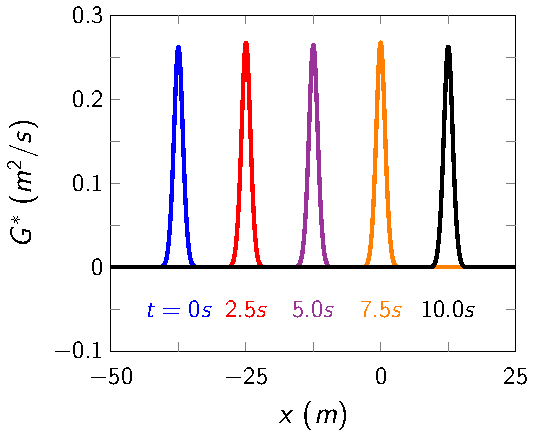
\includegraphics[width=0.8\textwidth]{./Pics/DryBed/Forced/G.pdf}
	\end{subfigure}
\end{figure}
	
\end{frame}

\begin{frame}{Modify Equations}
		\begin{align*}
		& \frac{\partial h}{\partial t} + \dfrac{\partial (uh)}{\partial x} = S_h^* ,  \\ \nonumber \\
		\begin{split}
		\frac{\partial G}{\partial t}  + \frac{\partial}{\partial x} \left( {u} G + \frac{gh^2}{2} - \frac{2}{3}h^3 \left[\frac{\partial {u}}{\partial x}\right]^2 + h^2 {u}\frac{\partial {u}}{\partial x}\frac{\partial b}{\partial x} \right) \\ + \frac{1}{2}h^2 {u} \frac{\partial {u}}{\partial x} \frac{\partial^2 b}{\partial x^2}  - h {u}^2\frac{\partial b}{\partial x}\frac{\partial^2 b}{\partial x^2} + gh\frac{\partial b}{\partial x} = S_G^* .
		\end{split}
		\end{align*}
		$S_h^*$ and $S_G^*$ are just the LHS  with the quantities replaced by their associated chosen function.
		% We solve the LHS using our method and add in the source terms on the RHS analytically.
\end{frame}

\begin{frame}{Results}
\begin{figure}[ht]
	\includemovie[
	poster,
	text={}
	]{6cm}{6cm}{Final.mp4}
\end{figure}
	
	%animate!!
\end{frame}


\begin{frame}{Modified Equations Validation Conclusions}
\begin{itemize}
	\item Very strong test as all terms must be accurately approximated
	\item Only source of error is the method
\end{itemize}
\end{frame}

	
\begin{frame}{Experimental Data}
	\begin{figure}
		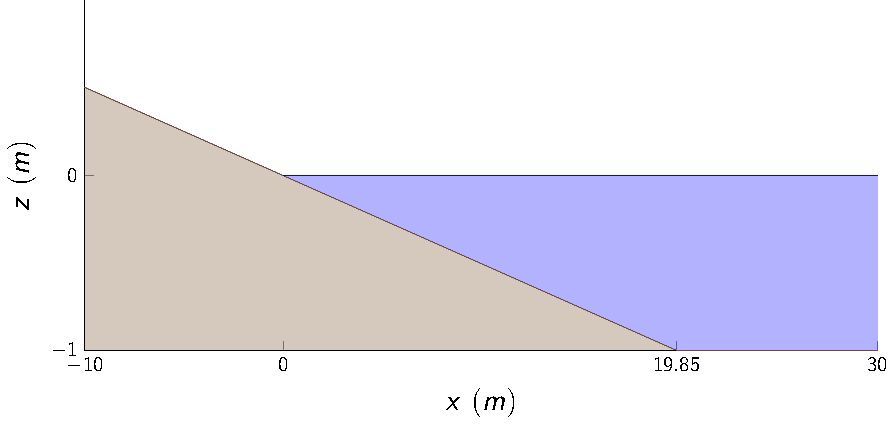
\includegraphics[width=1\textwidth]{./Pics/DryBed/Syn/WavetankArtificalPres.pdf}
	\end{figure}
\end{frame}

\begin{frame}{$t=30s$}
	\begin{figure}
		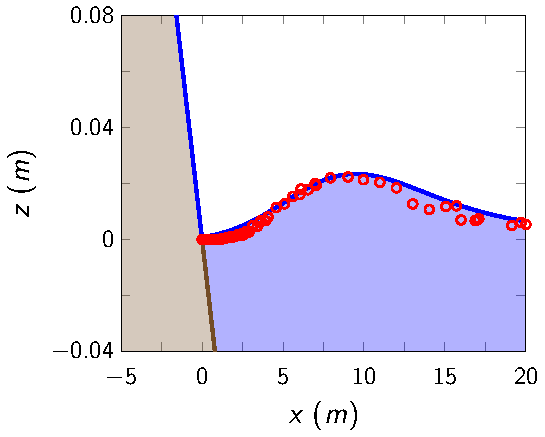
\includegraphics[width=0.8\textwidth]{./Pics/DryBed/Syn/t=30s.pdf}
	\end{figure}
\end{frame}

\begin{frame}{$t=40s$}
	\begin{figure}
		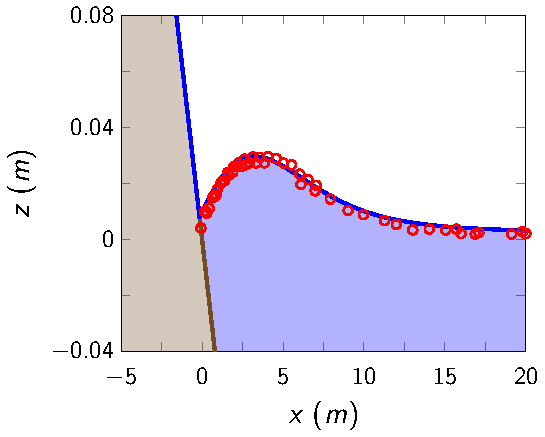
\includegraphics[width=0.8\textwidth]{./Pics/DryBed/Syn/t=40s.pdf}
	\end{figure}
\end{frame}

\begin{frame}{$t=50s$}
	\begin{figure}
		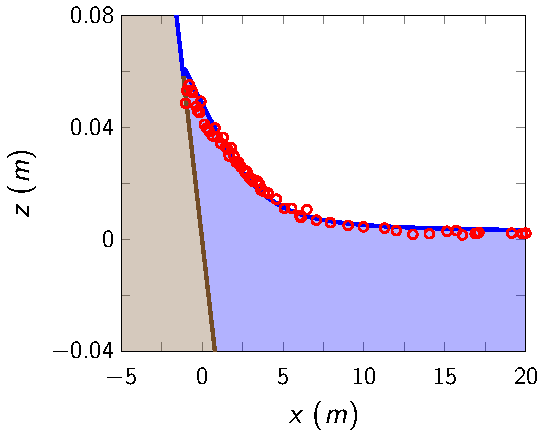
\includegraphics[width=0.8\textwidth]{./Pics/DryBed/Syn/t=50s.pdf}
	\end{figure}
\end{frame}

\begin{frame}{$t=60s$}
	\begin{figure}
		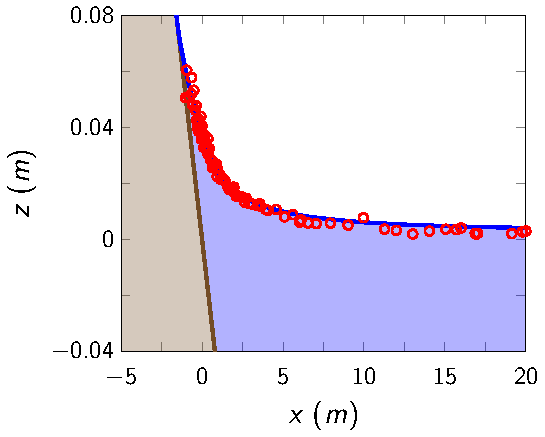
\includegraphics[width=0.8\textwidth]{./Pics/DryBed/Syn/t=60s.pdf}
	\end{figure}
\end{frame}

\begin{frame}{$t=70s$}
	\begin{figure}
		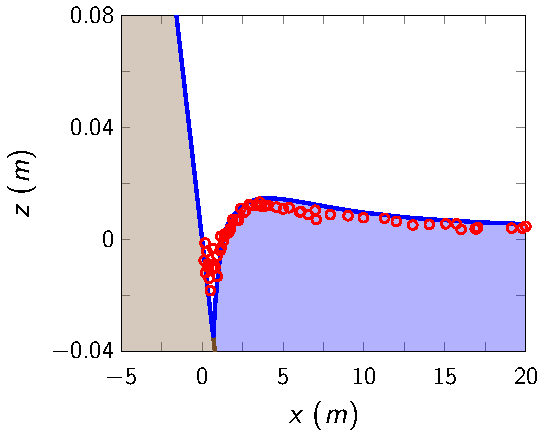
\includegraphics[width=0.8\textwidth]{./Pics/DryBed/Syn/t=70s.pdf}
	\end{figure}
\end{frame}
\begin{frame}{Experimental Validation Conclusions}
	\begin{itemize}
		\item Demonstrates agreement of computational model and physical process
		\item Many sources of errors
	\end{itemize}
\end{frame}

\begin{frame}{Progress}
	\begin{itemize}
		\item[2D:] 1D method that extends well to 2D \checkmark
		\item[Robust:] Validation for steep gradients in free surface \checkmark
		\item[Robust:] Inclusion and validation of dry beds \checkmark
	\end{itemize}	
\end{frame}

\begin{frame}{Conclusions}
	\begin{itemize}
		\item Developed a Robust Computational Model from the 1D Serre equations for the 2D water wave problem
	\end{itemize}
	\begin{figure}
		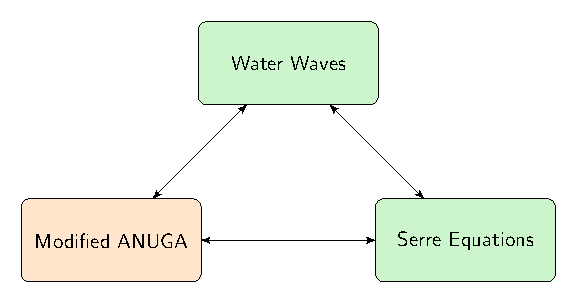
\includegraphics[width=\textwidth]{./Pics/ModelDiagrams/FlowChartSerre12G3O.pdf}
	\end{figure}
\end{frame}


\begin{frame}[allowframebreaks]
	\frametitle{References}
	\bibliographystyle{apalike}
	\bibliography{bibliography.bib}
\end{frame}

\end{document}